\section{Approach}
\label{sec:approach} To identify commonsense causality between two
statements, our framework includes i) a network of causal relations
between words that is extracted from a large web corpus; ii) a
metric to compute causal strength between any two words using this
network; iii) a heuristic method to extract intra-sentence events
that contain causality; and iv) a simple algorithm for aggregating
the causal strengths between words and events to compute the overall
causality score between two sentences. Next, we describe these
components.
%Our causality model presents a causal strength metric to quantify
%causality between any two text spans by constructing a term-based causal network
%from large web corpus.
%
%In this section, we first describe the causal network, then propose a causality
%quantify method. Though, our causality model can measure causality between any
%two text spans, when text spans are sentences, we particularly present a light
%weighting pattern by extracting intra-sentence events whose intuition is
%benefiting from implicit causality within them.
%(*or We detect the intra-sentence event which enhances causal relation
%and use the score from causal network to do the common sense reasoning.*)
%Finally, we combine our causality metric with light weighting pattern
%to formulate an algorithm which can be used for commonsense causal reasoning.
\subsection{Causal Network}
\label{sec:network}
Causality exists in natural language sentence and can be identified by
linguistic patterns known as {\em causal cues}~\cite{ChangC04}.
%We propose an easy way to automatically extract
%those causal pairs from web corpus.
%It is obvious that we can always distinguish
%cause and effect spans within sentences implied causality by properly designing
%casual cues.
For example, \textit{``A cause B''} is an intra-sentence causal
cue where \textit{A} is a text span that represents the cause
and \textit{B} is a span that represents the effect.
\tabref{tab:cue} shows all 53 intra-sentence and inter-sentence
causal cues used in this work.
We extract all such patterns from a large
web corpus, and after lemmatization, pair each word in $A$ with each word
in $B$ to form a list of \textit{causal pairs}.
These pairs form a {\em directed} network of causal relations. Each
node in this network is a lemmatized word, while a directed edge between two words
$u$ and $v$ indicates a causal relation, e.g., $u \rightarrow v$.
In this process, only pairs involving nouns, verbs,
adjectives and adverbs from WordNet are included in the network.
A fragment of the causal network with three words in the network is
shown in \figref{fig:causalnet}.
%We give more reasonable causality score
Each edge is annotated with the {\em causal strength}, which will be defined
next.

\begin{table*}[th]
\centering
\caption{53 Causal cues. \textit{A} is a cause span, and \textit{B} is an effect span.
DET stands for a/an/the/one. BE stands for is/are/was/were.}
\label{tab:cue}
\small
\begin{tabular}{|l l l|l l l|}
\hline \multicolumn{3}{|c|}{intra-sentence} & \multicolumn{3}{c|}{inter-sentence}\\
%\hline intra-sentence cue & inter-sentence cue  \\
\hline \hline
%\hline & \\
%\hline &\\
%A cause B & B caused by A & A induce B & If A, then B & A, hence B & A, thus B\\
A lead to B & A leads to B & A led to B & If A, then B& If A, B & B, because A \\
A leading to B & A give rise to B & A gave rise to B & B because A & B because of A & Because A, B \\
A given rise to B & A giving rise to B & A induce B & A, thus B & A, therefore B & B, A as a consequence \\
A inducing B & A induces B & A induced B & Inasmuch as A, B & B, inasmuch as A & In consequence of A, B \\
A cause B & A causing B & A causes B & B due to A & Due to A, B & B in consequence of A \\
A caused B & B caused by A & A bring on B & B owing to A & B as a result of A & As a consequence of A, B\\
A brought on B & A bringing on B & A brings on B & A and hence B & Owing to A, B& B as a consequence of A\\
B result from A & B resulting from A &  B results from A & A, hence B & A, consequently B & A and consequently B\\
B resulted from A & \multicolumn{2}{l|}{the reason(s) for/of B BE A} & \multicolumn{3}{|l|}{A, for this reason alone , B} \\
DET effect of A BE B &\multicolumn{2}{l|}{A BE DET reason(s) of/for B} & & & \\
\hline
\end{tabular}
\end{table*}

We choose to extract word pairs in a rather simplistic way, without deeper
syntactic analysis, because i) we opt for breadth in the causal knowledge
hence the input corpus is extremely large (around 10TB), and consequently
deep parsing of the text becomes prohibitive; and ii) the sheer quantity of
the word pairs thus obtained provides excellent statistics for us to
distinguish true causal pairs against false ones.

%In our causality model, we treat each term pair as a causal pair.
%For one term pair $(u,v)$, having the relation u causes v,
%we introduce the definition of role type of the words u and v.
%So we define causal pair for term pair $(u,v)$ as $\langle C(u)\rightarrow
%E(v)\rangle$, where $C(.)$ denotes the cause role and $E(.)$ denotes the effect role,
%shows the cause/effect role u and v plays in such causal relation.
%
%We prune our dataset by dumping the stop words, which means common but short function words such as a, an, to,
%and low frequency words.
%Lemmatization are also done to group the different inflected forms of
%a word together.
%After computing the causal strength illustrated in
%\figref{sec:causalstrength}, we build our causal network.

\begin{figure}[th]
\centering
\epsfig{file=causalnet.eps, width=0.6\columnwidth}
\caption{A fragment of causal network}
\label{fig:causalnet}
\end{figure}

%Intra-sentence causal cues are like "cause", "lead to" and "result from"
%while inter-sentence causal cue is like "because" and "if...then...".
%Patterns we used are strong and comprehensive enough to indicate the causal relations.
%Some cues are shown in \tabref{tab:cue} and we totally defined $53$
%causal cues like this.
%Since we also distinguish the active and passive voice,
%we have the confidence that the part A contains the cause evidence
%as well as part B contains the effect evidence.
%After that, we connect each word in part A to that in part B,
%and get the term pairs with frequencies corresponding different
%patterns besides the sum of those frequencies.
%


%(*The edges of the graph is attached with the causal strength of two words.*)
%It can be seen as a directed graph where an arrow starts from a cause term and
%ends to an effect term.
%We use term pairs identified with cause/effect roles (\emph{causal pairs}) to
%construct our causal network.
%
\subsection{Causal Strength Computation}
\label{sec:causalstrength}
%As we use the role type to distinct cause/effect roles in one term pairs,
%there is still a lack of metric so that we can compare the causal strength among
%pairs.
%As a result, we design our causal strength metric and assign scores to the causal pairs.
%
%We introduce two types of roles for term pair $(u,v)$ to present a new
%definition of causal pair $\langle(u,c)\rightarrow(v,e)\rangle$, where $(u,c)$
%denotes that word $u$ represents cause role and $(v,e)$ denotes that word $v$
%represents effect role. where $u,v$ denote words in our corpus and $c,e$ denote
%cause/effect role respectively in one word pair.
%To simplify the formulation, we just replace $[u,c]$, $[v,e]$,
%$\langle[u,c],[v,e]\rangle$ with $u,c$, $v,e$, and $(u,c,v,e)$ respectively.

%\ZY{
Our causal strength metric can be seen as a variant of
PMI (Pointwise Mutual Information), computed over a causal pair $u \rightarrow
v$ and their frequencies extracted from the web corpus. We can omit the
usual logarithm for ranking word pairs \cite{Washtell09:CWW}
%}.
%Maybe the easiest way to distinct cause/effect roles is encoding this
%information in causal cues.
%That's the strategy adopted in our causality model.
%The original PMI is defined as follows:
%\begin{equation}
%PMI(u,v) = \frac{P(u,v)}{P(u)P(v)}
%\end{equation}
%where $P(u,v)$ is the probability of observing words $u$ and $v$, in that
%% order, in the same sentence~\cite{Church:assoc}.
To distinguish between a cause word and
an effect word, we write $u_c$ to denote $u$ appeared in the 
cause span in the cue patterns, and $u_e$ to denote $u$ appeared 
in the effect span in the cue patterns.
We derive the {\em causal strength} between two words as follows.
First we define the joint probability of a causal pair as:
\begin{align}
P(u \rightarrow v) &= P(u_c~|~v_e)P(v_e) \nonumber \\
 &= P(v_e~|~u_c)P(u_c) \label{eq:joint}
\end{align}
Then, we define a basic causal strength score $CS_0$ over the causal pairs as:
\begin{align}
CS_0 (u,v) &= \frac{P(u \rightarrow v)^2}{P(u_c)^2 P(v_e)^2} \nonumber\\
 &= \frac{P(u_c ~|~ v_e)P(v_e) \times P(v_e~|~u_c)P(u_c)}{P(u_c)^2 P(v_e)^2} \nonumber\\
 &= \frac{P(u_c ~|~ v_e)P(v_e | u_c)}{P(u_c)P(v_e)}
\label{eq:pmi2}
\end{align}

The intuition for $CS_0$ is to take advantage of the conditional
probability in both directions in \eqnref{eq:joint}.
We further generalize \eqnref{eq:pmi2} to include two tunable parameters
$\alpha$ and $\beta$ that have been effectively adopted for PMI
to penalize high-frequency terms~\cite{Church:assoc}.
\begin{equation}
CS(u,v) = \frac{P(u_c~|~v_e) P(v_e~|~u_c)}
{P^\alpha(u_c)P^\beta(v_e)}\label{eq:cpmi}
\end{equation}
where
$P(u_c~|~v_e)$ and $P(v_e~|~u_c)$ can be computed as follows:
\begin{equation}
P(u_c~|~v_e) = \frac{f(u \rightarrow v)}{\sum_{w\in W}
f (w\rightarrow v)}
\end{equation}
\begin{equation}
P(v_e~|~u_c) = \frac{f(u\rightarrow v)}{\sum_{w\in W}
f(u\rightarrow w)}
\end{equation}
Here, $f(u\rightarrow v)$ is frequency of observing the causal pair
from the corpus; $W$ is the set of all words in the causal network.
%Since both cause and effect roles are important for causality identification, it
%is reasonable to treat two roles within a causal pair equally when we
%calculate causal strength. Therefore, we use same $\alpha$ for both roles as
%penalty for high frequency terms.
We compute the causal strength between every pair of words in the causal network
according to \eqnref{eq:cpmi}. Where an edge is missing in the network, we assign
a causal strength of zero.
%For our target problem, $\alpha$ and $\beta$ were empirically tuned to 0.5, which was consistently observed as an effective value for general PMI metrics in~\cite{}.


\subsection{Intra-sentence Event Enhancement}
\label{sec:eventBoost}
%For causality between two sentences, we can also utility its syntactic
%structure knowledge.
Causality, in reality, exists between events, which are often
expressed in more than one word. If we can detect events in a
sentence, which are more likely to be involved in causal relations,
we can reduce the noises produced by other unimportant words which
are outside the events in that sentence and increase the accuracy of
the causal reasoning. Moreover, it is observed that an event that
contains causality between the words within itself appears to be
more probable to cause other events in a ``ripple effect''. Consider
these two examples.
\begin{itemize}
\item They \emph{cut} the hamburger in \emph{half}.
\item The man \emph{grew} \emph{old}.
\end{itemize}
Events \emph{cut} $\rightarrow$ \emph{half} and \emph{grow}
$\rightarrow$ \emph{old} exhibit positive causality. These events
usually contain a strong action verb, which may lead to other
consequences. In this subsection, we seek to identify events in the
input sentences of commonsense causal reasoning task, and boost
their weights in the computation of causal strength between two
sentences.
%
% Though we only extract term-to-term causal pairs,
%events concerning causal relation are usually not one word.
%As a result, when dealing with the commonsense reasoning,
%we extract the events from sentences to enhance the causal evidence.
%There are two reasons of doing this.
%One is that, causality usually exists between events.
%\cite{} says that event contains most information of \emph{change of state}.
%So event extraction can help us exclude noisy words in sentence
%which are not so important for causality recognition and focus on the real import words.
%The other one is because we observed that causality does not only exist between two sentences,
%it also exists in one sentence, for which reason $PMI$ makes sense.
%For example, sentences like ``They \emph{cut} the hamburger in
%\emph{half}.'', ``The man \emph{grew} \emph{old}.'' We make use
%of the intra-sentence implicit causality such as `cut$\rightarrow$half`,'grow$\rightarrow$old' to get better result.

To extract the events, which we treat as a set of words here,
we parse the input sentence into dependency tree,
and identify verbs, their direct objects as well as some of
their significant modifiers.
For example, from ``I knocked on my neighbor's door,'' we can extract an event
{\em knock-neighbor-door}.
Only nouns, verbs, adjectives and adverbs are extracted
as part of an event. It is possible to extract multiple events from a sentence,
in which case we keep the one closest to the root of dependency tree.
Algorithm \ref{algo:events} gives the details of this process, while $rel(u)$
denotes dependency relation of node $u$, the distance between an event to the
root is calculated as:
\begin{equation}
\rm{RootDist}(e) = \frac{\sum_{w \in e} \rm{dist}(Root, w)}{|e|}
\end{equation}

%For those events have overlaps, we kept the most compact one gather around the root. We also
%guarantee that extracted events only contain ``nouns'',``verbs'',``adjectives''
%and ``adverbs''.
\begin{algorithm}[th]
\caption{Events Extraction}
\label{algo:events}
\begin{algorithmic}[1]
\begin{small}
\State Parse sentence $S$ to obtain dependency parse tree $T$
\State Define dependency relation set: \\
\quad \quad $R \leftarrow \{dobj, pobj, amod, nn, acomp, ccomp\}$ 
\State $EventSet \leftarrow \{\}$
\State $event \leftarrow \{\}$
\For {node $u \in T ~ \land ~ rel(u) \in R$}
\State $event$ $\leftarrow$ $event$ $\cup \{u\}$
\While {$u$ has a dependency head $v$}
\State $event \leftarrow event \cup \{v\}$
\If {$v$ is a verb}
\State $EventSet \leftarrow EventSet \cup \{event\}$
\State $event \leftarrow \{\}$
\State break;
\Else { $u \leftarrow v$}
\EndIf
\EndWhile
\EndFor
\For {$e \in EventSet$}
\If { $\exists e^{'} \in EventSet, e^{'} \subseteq e$ }
\State remove $e^{'}$ from $EventSet$
\EndIf
\If {$\exists  e^{'} \cap e \ne \emptyset$ }
\State $e^{*} = \argmin_{e} RootDist(e)$
\State remove $e^{'}, e$ from $EventSet$
\State $EventSet \leftarrow EventSet \cup \{e^{*}\}$
\EndIf
\EndFor
\end{small}
\end{algorithmic}
\end{algorithm}

\begin{figure}[th]
\centering
\epsfig{file=causeEvent.eps, width=0.6\columnwidth}
\caption{Weights in an event in a cause sentence}
\label{fig:causeEvent}
\end{figure}

\begin{figure}[th]
\centering
\epsfig{file=effectEvent.eps, width=0.32\columnwidth}
\caption{Weights of event in an effect sentence}
\label{fig:effectEvent}
\end{figure}

For the words in the extracted events, we perform the intra-sentence
enhancement to strengthen the causal signal of some important words.
Recall that in commonsense causal reasoning, we need to compute the
overall causal strength between the premise and an alternative. It
is known {\em a priori} whether the premise is a cause or an effect.
Therefore, when we extract event from an input sentence, which can
be either the premise or the alternative, we know whether the event
is to be a cause, which we call {\em cause event}, or an effect,
which we call {\em effect event}. We formulate events as
light-weight patterns to refine the causality score between two
sentences. In simple terms, it is a process of boosting weights of
cause words in cause events and effect words in effect events, by
assigning weights to words according to the the number of outgoing
and incoming edges. In \figref{fig:causeEvent}, which shows an event
{\em knock-neighbor-door} extracted from a cause sentence, there are
originally six edges among the three words, each carries a \emph{CS}
score between the two adjacent words. For each pair of words in this
sub-graph, we remove the edge with a smaller score, and effectively
retain three edges (marked by solid lines) as a result. Then for
each word, we count the number of {\em outgoing} edges (since this
is a cause event), which acts as the weight for that word. In this
case, {\em knock} has weight 2, {\em neighbor} has weight 0, while
{\em door} has a weight of 1. Similarly weights can be computed by
counting the number of {\em incoming} edges for the effect event
{\em leave-house} in \figref{fig:effectEvent}.

In the next subsection, when we compute the causal strength score between two sentences,
the cause strength between any two words will be boosted by their respective weights
which are computed here.
%
%For example, we extract ``\emph{predict} \emph{high} \emph{temperature}''
%(*need to change*)as cause event, the light weighting pattern is shown as
%\figref{fig:causeEvent}.
%We extract `` \emph{cast} \emph{shadow} '' as effect event , the light weighting
%pattern is shown as \figref{}.
%
%which contains only two words, we compare two causal strength
%values modeled with $\alpha$-\textit{causality PMI}. If
%$\textit{PMI}_{\alpha\textit{-causality}}[\langle C(w1)\rightarrow
%E(w2)\rangle]$  $\textit{PMI}_{\alpha\textit{-causality}}[\langle
%C(w2)\rightarrow E(w1)\rangle]$ and specify the direction in such event.
%Like the example shown above, we compare the
%$\textit{PMI}_{\alpha\textit{-causality}}[\langle C(\textit{cut})\rightarrow
%E(\textit{half})\rangle]$ score of ``cut $\rightarrow$ half'' and
%"half$\rightarrow$cut" and then confirm that the direction comes from "cut" and
%goes to "half".
%
%(*How we formulate the light pattern within events?*)
%
%For events in cause sentences, we count the number of
%outgoing edges of one word as its weight in the event.
%And for events in effect sentences,
%we count the number of incoming edges of one word as its weight in the event.
%This is because words with more outgoing edges in cause sentence tend to be the initial reason of the event,
%which is the same for words with more incoming edges in effect sentence.
%By doing so, we strengthen the inner events and tune weights for event words.
%
%If there isn't a strong inner causality structure some events,
%boosting process based on causality score will usually lead to boosting verbs
%weights more of that event which is also reasonable, since verbs usually the
%most important of role of one sentence/event.

\subsection{Commonsense Causal Reasoning}

To compute whether alternative $a_1$ or $a_2$ is more plausible
w.r.t. the premise $p$, we need to compare the overall causal
strength $CS_T(p, a_1)$ and $CS_T(p, a_2)$, assuming $p$ is asking
for an effect. The overall causal strength score from text $T_1$ to
text $T_2$ is computed as:
\begin{align}
CS_T(T_1,T_2)&=\frac{1}{|T_1|+|T_2|}\sum_{u \in T_1}\sum_{v \in T_2}
(1+ \omega(u))(1+ \omega(v))   \nonumber \\
& \delta(u, v) CS(u, v)
\label{eq:csall}
\end{align}
where $\omega(w)$ is the weight given by event enhancement for word $w$,
and $\delta(u,v)$ is a penalty factor for the semantic ambiguity of $u$ and
$v$, defined as:
\begin{equation}
\delta(u,v) = \frac{1}{\#senses(u)+\#senses(v)}
\end{equation}
where $\#senses(u)$ denotes number of WordNet synsets word $u$ belongs to,
which indicates how ambiguous $u$ can be.
We penalize ambiguous words in the same spirit as the inverse document frequency
(IDF) in information retrieval. The reason is when an ambiguous word $u$ is paired
with every other word in another sentence, the causal strengths calculated for
each pair may be due to different context and different senses of $u$ and thus
produce unreliable overall causal strength.
Suppose we change the premise in \secref{sec:intro} to
\begin{itemize}
\item[] Premise: {\em My neighbor is a doctor}.
\end{itemize}
When computing the causal strength with Alternative 2, since the
word \emph{leave} is ambiguous, it means ``depart'' when paired with
\emph{neighbor}, whereas it means ``absence from duty (medical)''
when paired with \emph{doctor}.

%\ZY{
In our causality model, we treat each cause word as a \emph{trigger} and each
effect word as a \emph{response}.
We modeled one-to-many relationship between triggers and responses, which
means one trigger can cause many responses, similarly one response can be caused
by many triggers.
That's the reason we normalize causality score by $|T_1|+|T_2|$ not
$|T_1|\times|T_2|$ presented in previous papers. 
%}

%\begin{align}
%CS_{\rm max}(T_1,T_2)&=\frac{1}{|T_1|}\sum_{t_1 \in T_1}w(t_1) \times\nonumber\\
%&w(\argmax_{t_2 \in T_2}{PMI}^2_{\text{causality}}(t_1, t_2)) \times\nonumber\\
%&\delta(t_1, \argmax_{t_2 \in T_2}{PMI}^2_{\text{causality}}(t_1, t_2)) \times  \nonumber\\
%&\left(\max_{t_2 \in T_2} {PMI}^2_{\text{causality}}(t_1, t_2)\right)
%\label{eq:csmax}
%\end{align}
%


%
%
%We've already penalized causality score of high frequency terms when we
%calculate $\alpha$-causality PMI. And since our
%causal network is term based, some terms with many senses tends to form many
%false causal pairs with other terms. For example, when term \emph{bank} means
%financial organization, it can form correct causal pair such as $\langle
%C(\rm{bank})\rightarrow E(\rm{loan})\rangle$. But if \emph{bank} means river
%side, it is more reasonable to form causal pair $\langle
%C(\rm{bank})\rightarrow E(\rm{river})\rangle$. So we need to discounting for
%terms ambiguity by calculating ambiguity weight for causal pair $u,v$ as following.
%First of all, we set each term of cause/effect segments to be $1$,
%which means we consider all terms have same significance in each sentence.
%Then we step into the tuning process, boosting weights for events words in
%,utilize inner causality structure to form a light weighting pattern within
%sentence.
%
% \begin{algorithm}[th]
% \caption{Causality Calculation Between Text Segments}
% \label{algo:causality}
% \begin{algorithmic}[1]
% \Function{Causality}{$T_{cause},T_{effect}$}
% \State $S \leftarrow 0$
% \For{$t_1 \in T_{cause}$}
% \For{$t_2 \in T_{effect}$}
% \State $ amb \leftarrow \left. 1 \middle / (\#senses(t_1)+\#senses(t_2))
% \right.$ \State $ S \leftarrow S + amb*PMI_{\alpha\textit{-causality}}(t_1,t_2) $
% \EndFor
% \EndFor
% \State $E_1 \leftarrow ExtractEvent(T_{cause})$
% \State $E_2 \leftarrow ExtractEvent(T_{effect})$
% \State $W_1 \leftarrow Tuning(E_1)$
% \State $W_2 \leftarrow Tuning(E_2)$
% \For{$e_1 \in E_1, w_1 \in W_1$}
% \For{$e_2 \in E_2, w_2 \in W_2$}
% \State $S \leftarrow S + w_1*w_2*PMI_{\alpha\textit{-causality}}(e_1,e_2)$
% \EndFor
% \EndFor
% \EndFunction
% \end{algorithmic}
% \end{algorithm}
%

%We can measure any two text segments using our causality model.
%For two text segments $T_1$ and $T_2$,
%where $T_1$ is supposed to be the candidate cause segment
%and $T_2$ be the effect one.
%we assume that the number of useful words in each segment is 4(denote u1, u2, u3, u4) and 3(denote v1, v2, v3)
%\figref{}.
%(as Figure [] shows).
%First we extract events from both segments,
%applying the intra-sentence event enhancement to get the additional weight for event word.
%So, in this practical problem,
%we get the local strength of the event word as the product of weight and global causal strength.
%Then, we connect words of $T_1$ to words of $T_2$ just as what we do to get the causal network pairs.
%The direction is from cause segment to effect segment.
%By summing up the causal strength of those pairs,
%we get the total causal strength from $T_1$ to $T_2$.
%After boosting weight for each term in $T_1, T_2$. We formulate term $t$ and
%its weight $w$ together as $(t,w)$. So now we can see $T_1,T_2$ as weighted text
%segments consists of such weighted terms.
%%The causality between two segments $T_1$ and $T_2$ is therefore computed as Figure [] shows:

%Commonsense casual reasoning is
%We pair up
%After properly modeling, we outperform state of the art by just simply
%pairing up all causal pairs together, sum up their causal strength
